\documentclass[12pt, a4paper]{article} %determina o tamanho da fonte, o tipo de papel e o tipo de documento.

\setlength{\parindent}{1.0 cm} %tamanho do espaço para começar o parágrafo.
\setlength{\parskip}{0.5cm} %tamanho do espaço entre os parágrafos.

%Aqui ficam os pacotes utilizados para formatação do documento de modo geral:

\usepackage[utf8]{inputenc} 
\usepackage{indentfirst} %Coloca espaços nos inícios de parágrafos automaticamente. 
\usepackage[brazilian]{babel} %
\usepackage{amsmath}
\usepackage[hmargin=3cm, vmargin=2.5cm, bmargin=2.5cm]{geometry}
\usepackage{multicol}
\usepackage{graphicx} %para poder inserir imagens
\usepackage{subfig}
\usepackage{booktabs} 
\usepackage{hyperref} %para poder adicionar links e hiperlinks
\usepackage{float} %para poder posicionar as imagens


\usepackage{listings} %para poder incluir códigos
\usepackage{xcolor}
\definecolor{codegreen}{rgb}{0,0.6,0}
\definecolor{codegray}{rgb}{0.5,0.5,0.5}
\definecolor{codepurple}{rgb}{0.58,0,0.82}
\definecolor{backcolour}{rgb}{0.95,0.95,0.92}
\lstdefinestyle{mystyle}{
    backgroundcolor=\color{backcolour},   
    commentstyle=\color{codegreen},
    keywordstyle=\color{magenta},
    numberstyle=\tiny\color{codegray},
    stringstyle=\color{codepurple},
    basicstyle=\ttfamily\footnotesize,
    breakatwhitespace=false,         
    breaklines=true,                 
    captionpos=b,                    
    keepspaces=true,                 
    numbers=left,                    
    numbersep=5pt,                  
    showspaces=false,                
    showstringspaces=false,
    showtabs=false,                  
    tabsize=2,
    morecomment={l}[!],
    language=[77]Fortran,
}
\lstset{style=mystyle}

\begin{document} %começa alguma coisa,neste caso, o documento, sempre importante lembrar de colocar o \end{} para não dar erro 
	
	\begin{titlepage}
		\begin{center}
\Huge{Universidade de São Paulo}\\
\large{Instituto de Física de São Carlos}\\
\vspace{20pt}
\vspace{200pt}
\textbf{Lista 2}\\
\vspace{8cm}
		\end{center}

\begin{flushleft}
\begin{tabbing}
Pedro Calligaris Delbem 5255417\\
\end{tabbing}
\vspace{0.5cm}
Professor: Attilio Cucchieri\\		
		\end{flushleft}
	
		\begin{center}
			\vspace{\fill}
	Março de 2025	
		\end{center}
	\end{titlepage}

%####################################################################### SUMÁRIO
	\tableofcontents 
	\thispagestyle{empty}
	\newpage
%#########################################################################

\section{Finding roots}

    \subsection{Exerc\'icio 1}

        Tarefa: Demonstrar que no m\'etodo de Newton-Raphson
        \begin{equation}
            x_{k+1} = x_{k} + \frac{f(x_{k})}{f'(x_{k})}
        \end{equation}
        a converg\^encia \'e quadr\'atica.

        Expandimos f(x) em torno de $x_{n} - r$ - onde r \'e a raiz de f(x) - e obtemos:
        \begin{equation}
            f(x_{n}) = f(r) + f'(r)(x_{n} - r) + \frac{1}{2} f''(r)(x_{n}  - r)^2 + O(x_{n} - r)^3
        \end{equation}
        E como f(r) = 0, obtemos:
        \begin{equation}
            f(x_{n}) = f'(r)(x_{n} - r) + \frac{1}{2} f''(r)(x_{n}  - r)^2 + O(x_{n} - r)^3
        \end{equation}
        Expande-se, também, $f'(x_{n})$ e obtemos:
        \begin{equation}
            f'(x_{n}) = f'(r) + f''(x_{n} - r)(x_{n} - r) + O(x{n} - r)^2
        \end{equation}
        Substituindo em $x_{n+1} = x_{n} + \frac{f(x_{n})}{f'(x_{n})}$ obtemos:
        \begin{equation}
            x_{n+1} = x_{n} - \frac{f'(r)(x_{n} - r) + \frac{1}{2} f''(r)(x_{n}  - r)^2}{f'(r) + f''(x_{n} - r)(x_{n} - r)}
        \end{equation}
        Subtraindo r de ambos os lados:
        \begin{equation}
            x_{n+1} - r = x_{n} - r - \frac{f'(r)(x_{n} - r) + \frac{1}{2} f''(r)(x_{n}  - r)^2}{f'(r) + f''(x_{n} - r)(x_{n} - r)}
        \end{equation}
        Colocando o termo $x_{n} - r$ em evid\^encia:
        \begin{equation}
            x_{n+1} - r = (x_{n} - r)\bigg[1 - \frac{f'(r) + \frac{1}{2} f''(r)(x_{n}  - r)}{f'(r) + f''(x_{n} - r)(x_{n} - r)}\bigg]
        \end{equation}
        Para $x_{n} - r$ pequeno, f''(r)$(x_{n} - r)$ \'e disprez\'ivel e assim o desprezamos no denominador - obtendo:
        \begin{equation}
            x_{n+1} - r = (x_{n} - r)\bigg[1 - \frac{f'(r) + \frac{1}{2} f''(r)(x_{n}  - r)}{f'(r)}\bigg]
        \end{equation}
        Isolando $x_{n} - r$:
        \begin{equation}
            x_{n+1} - r = -(x_{n} - r)^2\bigg[\frac{\frac{1}{2} f''(r)}{f'(r)}\bigg]
        \end{equation}
        Rearranjando:
        \begin{equation}
            r - x_{n+1} = (r - x_{n})^2\bigg[\frac{\frac{1}{2} f''(r)}{f'(r)}\bigg]
        \end{equation}
        Como $r - x_{n}$ \'e o erro cometido na n-\'essima itera\c{c}\~ao e $r - x_{n+1}$ \'e o erro cometido na n+1-\'essima itera\c{c}\~ao, temos que o erro da itera\c{c}\~ao n+1 \'e proporcional ao quadrado do erro da itera\c{c}\~ao n e portanto a converg\^encia \'e quadratica.

    \subsection{Exerc\'icio 2}

        Tarefa: Achar as ra\'zes das equa\c{c}\~oes $f(x) = x^2 - 5 = 0$ e $f(x) = 5x^3 - 5x - 24 = 0$ usando os m\'etodos de Newton-Raphson e da secante para diferentes chutes iniciais e diferentes condi\c{c}\~oes de converg\^encia.

        %C\'odigo Escrito:
        %\lstinputlisting[language=Fortran]{../L2-5255417-ex-2.f90}

        O c\'odigo foi compilado com o comando:
        \begin{verbatim}
            gfortran L2-5255417-ex-2.f90 -o L2-5255417-ex-2.exe
        \end{verbatim}

        Resultados:

        \begin{figure}[H]
            \centering
            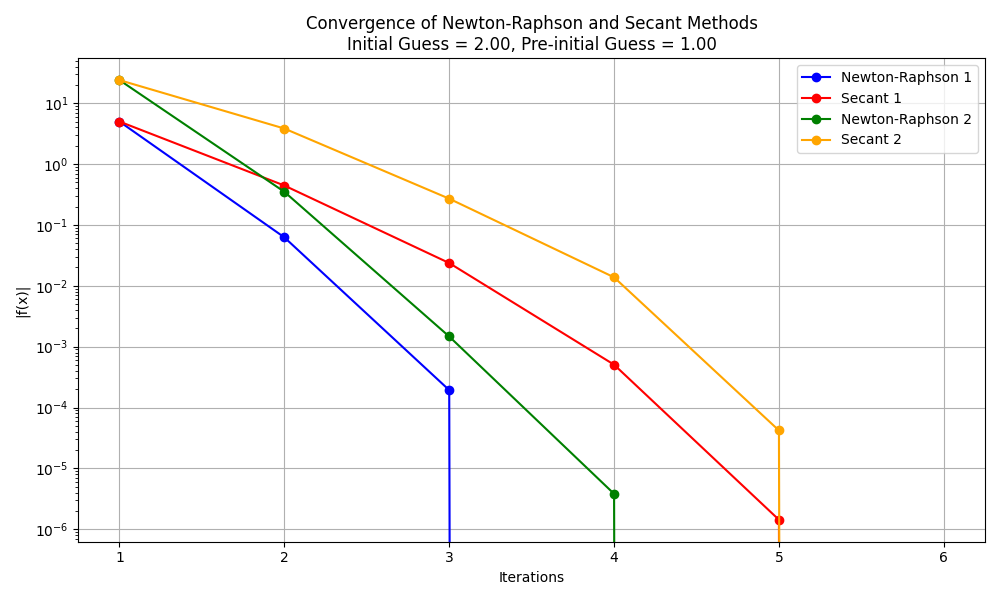
\includegraphics[width=0.8\textwidth]{../images/convergence-initial-20-preinitial-10.png}
            \caption{}
        \end{figure}

        \begin{figure}[H]
            \centering
            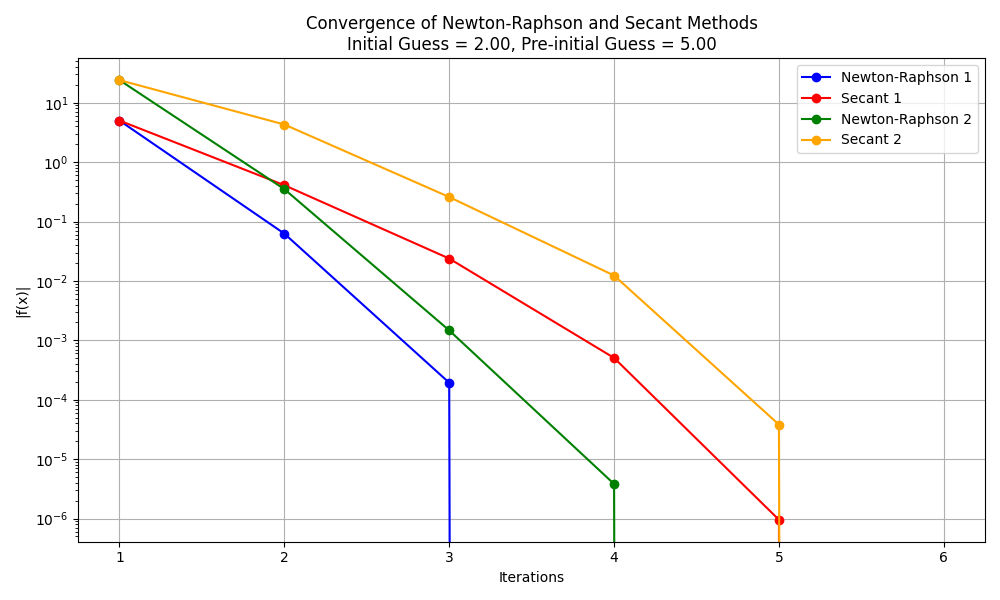
\includegraphics[width=0.8\textwidth]{../images/convergence-initial-20-preinitial-50.png}
            \caption{}
        \end{figure}
        
        \begin{figure}[H]
            \centering
            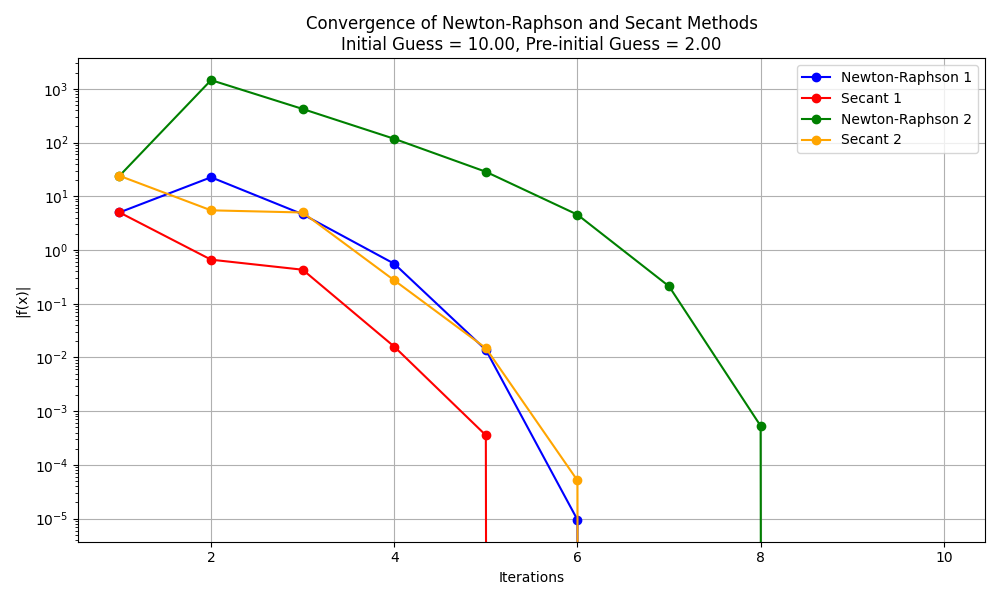
\includegraphics[width=0.8\textwidth]{../images/convergence-initial-100-preinitial-20.png}
            \caption{}        
        \end{figure}


        \begin{figure}[H]
            \centering
            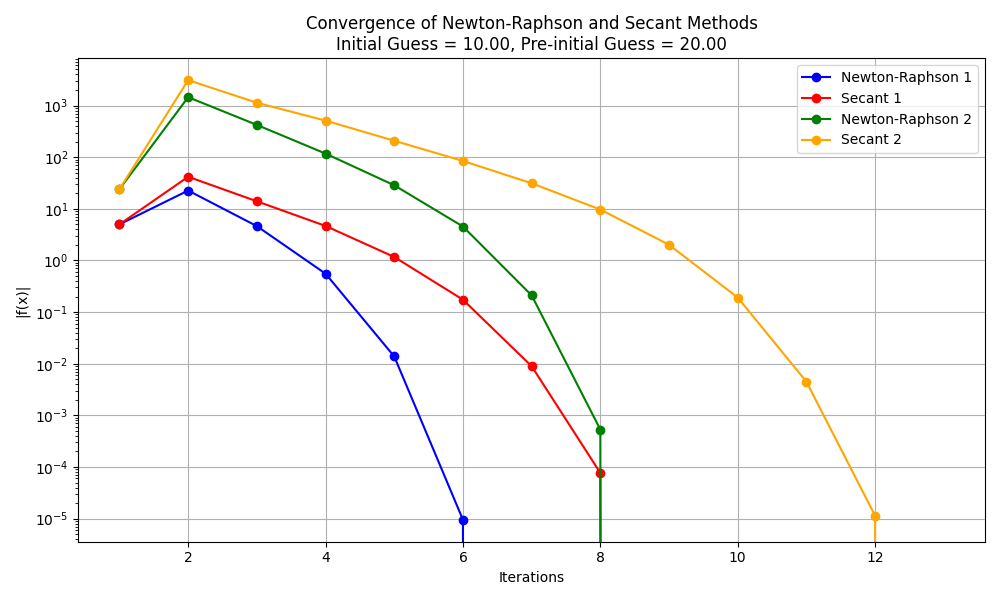
\includegraphics[width=0.8\textwidth]{../images/convergence-initial-100-preinitial-200.png}                
            \caption{}       
        \end{figure}

        \begin{figure}[H]
            \centering
            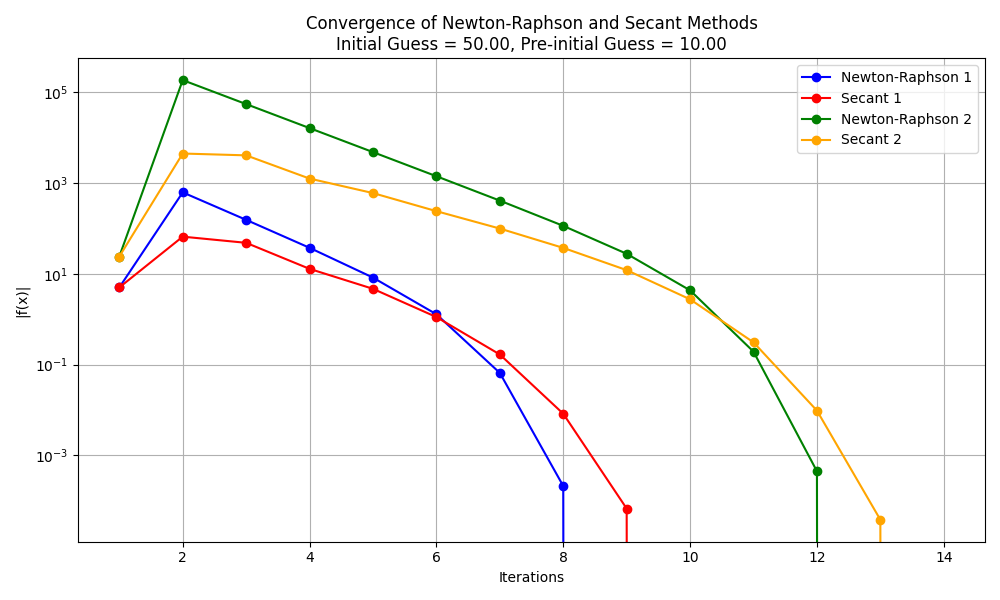
\includegraphics[width=0.8\textwidth]{../images/convergence-initial-500-preinitial-100.png}
            \caption{}        
        \end{figure}

        \begin{figure}[H]
            \centering
            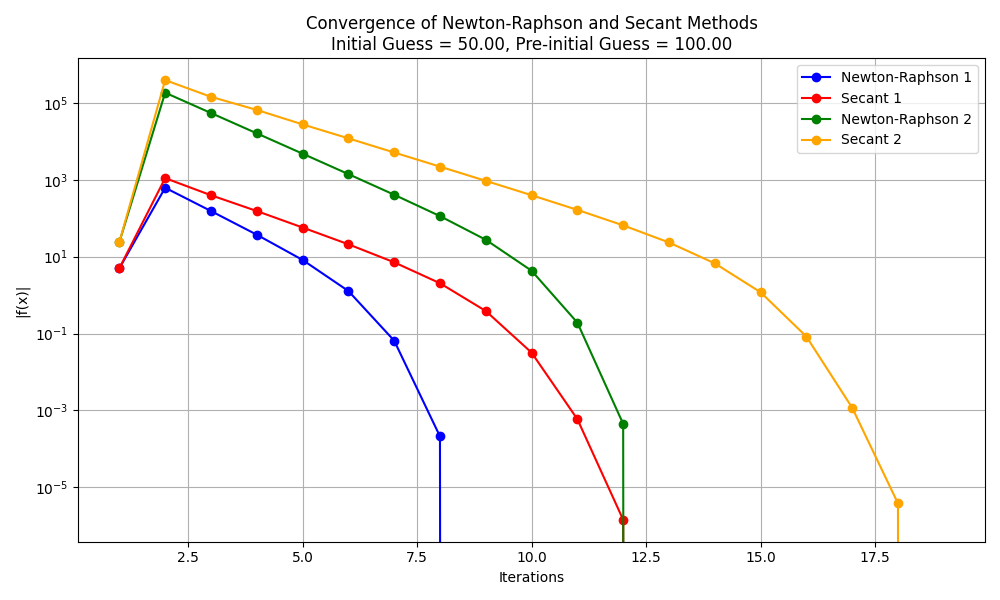
\includegraphics[width=0.8\textwidth]{../images/convergence-initial-500-preinitial-1000.png}
            \caption{}        
        \end{figure}

        As ra\'izes encontradas por ambos os m\'etodos foram: $f(x) = x^2 - 5$ = - 2.23606801 e $f(x) = 5x^3 - 5x - 24$ - 1.88367081
        Percebe-se que para bons chutes o m\'etdo da secante \'e mais eficiente, mas para chutes ruins o m\'etodo de Newton-Raphson \'e mais eficiente.

\section{Eigenvalues of the wave equation}

    \subsection{Exerc\'icio 3}

        Tarefa: Escreva a transforma\c{c}\~ao que permitem escrever a equa\c{c}\~ao de Schr\"odinger para os
        autoestados de uma part\'icula em um po\c{c}o infinito na forma
        \begin{equation}
            \frac{d^2}{dx^2}\psi(x) = -k^2\psi(x) \quad \text{com} \quad \psi(0) = 0 \text{ e } \psi(\infty) = 0
        \end{equation}

        Seja a equação de Schr\"odinger:
        \begin{equation}
                \left(-\frac{\hbar^2}{2m}\frac{d^2}{dx^2} + V(x)\right)\psi(x) = E\psi(x)
        \end{equation}
        Para o caso do po\c{c}o infinito a equa\c{c}\~ao pode ser escrita como:
        \begin{equation}
                -\frac{\hbar^2}{2m}\frac{d^2}{dx^2}\psi(x) = E\psi(x) \quad \text{com} \quad 0 \leq x \leq L 
        \end{equation}
        Para tornar adimensional, fazemos a transforma\c{c}\~ao $x \longrightarrow x/L$:
        \begin{equation}
                -\frac{\hbar^2}{2mL^2}\frac{d^2}{dx^2}\psi(x) = E\psi(x) \quad \text{com} \quad 0 \leq x \leq 1
        \end{equation}
        Rearranjando:
        \begin{equation}
            \frac{d^2}{dx^2}\psi(x) = -\frac{2mEL^2}{\hbar^2}\psi(x) \quad \text{com} \quad 0 \leq x \leq 1
        \end{equation}
        Note que $\frac{2mEL^2}{\hbar^2}$ \'e adimensional - como desejado. Ent\~ao, definimos $k^2 = \frac{2mEL^2}{\hbar^2}$ - obtendo:
        \begin{equation}
            \frac{d^2}{dx^2}\psi(x) = -k^2\psi(x) \quad \text{com} \quad \psi(0) = 0 \text{ e } \psi(\infty) = 0
        \end{equation}
        que \'e a equa\c{c}\~ao adimensional desejada.


    \subsection{Exerc\'icio 4}

        Tarefa: Escreva um c\'odigo para calcular os primeiros tr\^es n\'iveis de energia para o po\c{c}o de potencial infinito, usando o shooting method e as condi\c{c}\~oes de contorno $\psi(0) = 0$ e
        $\psi '(0) \neq  0$. Compare o resultado com a solu\c{c}\~ao exata.

        %C\'odigo Escrito:
        %\lstinputlisting[language=Fortran]{../L2-5255417-ex-4.f90}

        O c\'odigo foi compilado com o comando:
        \begin{verbatim}
            gfortran L2-5255417-ex-4.f90 -o L2-5255417-ex-4.exe
        \end{verbatim}

        Resultados:

    

    \subsection{Exerc\'icio 5}

        Tarefa: Escreva um c\'odigo para calcular os primeiros tr\^es n\'iveis de energia para o po\c{c}o de potencial infinito, usando o m\'etodo da secante e as condi\c{c}\~oes de contorno $\psi(0) = 0$ e
        $\psi '(0) \neq  0$. Compare o resultado com a solu\c{c}\~ao exata e com o resultado do exerc\'icio 4.

        %C\'odigo Escrito:
        %\lstinputlisting[language=Fortran]{../L2-5255417-ex-5.f90}

        O c\'odigo foi compilado com o comando:
        \begin{verbatim}
            gfortran L2-5255417-ex-5.f90 -o L2-5255417-ex-5.exe
        \end{verbatim}

        Resultados:
        

\end{document}